\documentclass[output=paper]{langscibook}

\graphicspath{{./figures/}}

\author{Mikhail Knyazev\orcid{0000-0003-4652-4144}\affiliation{Institute for Linguistic Studies RAS, Saint Petersburg;National Research University Higher School of Economics, Saint Petersburg}}
\title[Silent \textsc{have} needs revisiting]
      {Silent \textsc{have} needs revisiting: (Non-)possessive meanings with transitive intensional `need' in Russian}
\abstract{I discuss two `need'\,+\,NP constructions in Russian, namely (i) the more basic construction with a nominative theme and (ii) the underdescribed, highly colloquial construction with an accusative theme. Building on work on the semantics of possessive constructions, I show that the two constructions differ as to which semantic relations they can express. Specifically, the nominative construction can not only express the control relation (the most prototypical possessive relation), but also a variety of others, whereas the accusative construction is restricted to the control relation, as manifested in the animacy and concreteness restrictions associated with it. Based on previous work on intensional transitive verbs, I analyze both constructions as involving a concealed clausal complement with a silent \textsc{have} but extend this analysis by assuming that \textsc{have} selects an NP complement via a syntactically represented type-shifting operator, which encodes the respective semantic relations expressed in the construction. I further argue that the accusative construction incorporates the type-shifter for the control relation, thus accounting for its selectional restrictions, and tentatively suggest that this might also explain the accusative marking. Finally, I report the results of three acceptability rating studies testing the animacy and concreteness restrictions in the accusative construction.

\keywords{intensional transitive verbs, possession, case alternation, Russian, experimental syntax}
}


\begin{document}
\maketitle

\section{Introduction}\label{section-intro}

In standard \ili{Russian}, `need' with a nominal complement (compare to English \textit{I need a book}) is typically realized by the adjectival predicate \textit{nužen} `necessary', which takes a dative subject and a nominative theme controlling the number and gender agreement on the predicate (henceforth, the `need'\,+\,\textsc{nom} construction), as shown in \REF{need-nom}. In colloquial registers, `need' can also occur with accusative (sometimes genitive) themes without any clear truth-conditional difference, as shown in \REF{need-acc}. In this case `need' is realized by the non-agreeing (adverbial) form \textit{nužno}, identical to the neuter singular form, or by the non-inflecting impersonal predicate \textit{nado} (henceforth, the `need'\,+\,\textsc{acc} construction).\footnote{In what follows, \textit{nužno} and \textit{nado} are glossed as `adverbial' (\textsc{adv}) to highlight their non-verbal character, without any theoretical implications.}\largerpage

\ea
\ea \gll Mne nužn-a knig-a.\\
     me.\textsc{dat} necessary-\textsc{f.sg} book-\textsc{nom.sg}\\ \hfill `need'\,+\,\textsc{nom}
\glt `I need a book.'\label{need-nom}
\ex \gll Mne nužno / nado knig-u.\\
     me.\textsc{dat} necessary.\textsc{adv} {} necessary.\textsc{adv} book-\textsc{acc.sg}\\ \hfill `need'\,+\,\textsc{acc}
\glt `I need a book.'\label{need-acc}
\z \z

\noindent \textsc{acc} marking on the theme in the `need'\,+\,\textsc{acc} construction alternates with genitive marking for mass and plural nouns, as well as for some abstract nouns like `love', `happiness', etc., especially under negation, as shown in \REF{need-gen}. Henceforth, I will disregard examples with genitive marking and only discuss examples with \textsc{acc} themes.

\ea\label{need-gen}
\ea \gll Mne nado vod-y / sčast'-ja.\\
     me.\textsc{dat} necessary.\textsc{adv} water-\textsc{gen.sg} {} happiness-\textsc{gen.sg}\\
\glt `I need water/happiness.'
\ex \gll Mne ne nužno vod-y / podark-ov.\\
     me.\textsc{dat} \textsc{neg} necessary.\textsc{adv} water-\textsc{gen.sg}  {} present-\textsc{gen.pl}\\
\glt `I do not need water/presents.'
\z\z

\noindent The `need'\,+\,\textsc{nom} construction is stylistically neutral and is by far more frequent than the `need'\,+\,\textsc{acc} construction, which is highly colloquial and is sometimes considered non-standard by native speakers. Nevertheless, the `need'\,+\,\textsc{acc} construction occurs with a non-negligible frequency in the corpus.\footnote{In a study based on the \ili{Russian} National Corpus (RNC; \url{http://www.ruscorpora.ru}), I found 54 examples of `need'\,+\,\textsc{acc} with \textit{nužno} and 223 examples with \textit{nado} in the texts written after 1950. The results of this study are discussed in \citealt{Knyazev2020}.} There are further pragmatic differences between the two constructions, having to do with the subjective component in the meaning of `need'\,+\,\textsc{acc}. I disregard these differences in this paper (but see \citealt{Knyazev2020}).

The `need'\,+\,\textsc{acc} construction has been briefly discussed in the literature (see, e.g., \citealt[325--327]{Svedova1980}, \citealt[213]{Pesetsky1982}, \citealt[28]{Mikaelian.Roudet1999}), mostly in connection with other \textsc{acc}-assigning non-verbal predicates in \ili{Russian} such as \textit{žal'} `(it is a) pity', \textit{vidno} `(it is) visible', \textit{slyšno} `(it is) audible', and some others. To my knowledge, however, it has not received a detailed analysis so far and has never been systematically contrasted with the `need'\,+\,\textsc{nom} construction. Most strikingly, it is not mentioned in \citet{Harves2008} and \citet{Harves.Kayne2012}, which specifically address \ili{Russian} `need' with a nominal complement, a point to which I return in \sectref{section-acc-analysis}.

In \citet{Knyazev2020}, I discussed the semantic/distributional differences between the `need'\,+\,\textsc{nom} and the `need'\,+\,\textsc{acc} constructions, suggesting that `need'\,+\,\textsc{acc} has a more restricted distribution. Specifically, I argued that `need'\,+\,\textsc{acc} is restricted to the expression of concrete human possession, namely possession of concrete (manipulable) objects by human beings (which is sometimes metaphorically extended to abstract objects), which I referred to as the \textsc{concreteness} and the \textsc{animacy restrictions}. By contrast, the `need'\,+\,\textsc{nom} construction can express a wide variety of relations, including those that are not typically associated with possession.

In this paper, I review some of these findings but also situate them in a larger theoretical context, namely the literature on intensional transitive verbs, including, in particular, \citet{Harves2008} (and, to a smaller extent, \citealt{Harves.Kayne2012}), which is specifically dedicated to `need'\,+\,NP in \ili{Russian}. My goal is to show how these findings lead to a revision of the silent \textsc{have} analysis proposed by \citet{Harves2008} for the `need'\,+\,\textsc{nom} construction and also how this analysis can be extended to the `need'\,+\,\textsc{acc} construction (which \citeauthor{Harves2008} does not discuss), in a way that can capture its semantic restrictions.

The account I propose heavily relies on the recent semantic account of the English transitive `need' construction proposed in \citet{Zaroukian.Beller2013} (which is, in turn, strongly influenced by \citealt{Vikner.Jensen2002}). The particular importance of \citet{Zaroukian.Beller2013} is that it explicitly deals with the semantic variability in transitive `need' (which is rarely discussed in the literature) as well as proposes a compositional account of this variability.

The second goal of this paper is to present the results of three formal acceptability judgment studies aimed at investigating the proposed animacy and concreteness restrictions using methods of experimental syntax (see \citealt{Sprouse.Hornstein2013}). Somewhat unexpectedly, these studies failed to provide direct support for the hypothesized restrictions. I offer some speculations as to why these negative results might have been obtained and make some methodological suggestions for future research.

The paper is structured as follows: In \sectref{section-background}, I give an overview of the discussion of the `need'\,+\,NP construction in the literature on intensional transitive verbs, starting from the ``standard'' silent \textsc{have} analysis of `need'\,+\,NP (\sectref{section-silent-have}), then turning to some problematic examples with apparently non-possessive relations (\sectref{section-problematic}) and, finally, presenting \citeauthor{Zaroukian.Beller2013}'s \citeyearpar{Zaroukian.Beller2013} semantic account of `need'\,+\,NP (\sectref{section-zaroukian}). In \sectref{section-nom}, I turn to the `need'\,+\,\textsc{nom} construction in \ili{Russian}, first briefly presenting \citeauthor{Harves2008}'s \citeyearpar{Harves2008} account (\sectref{section-harves}), then discussing semantic relations expressed in this construction (\sectref{section-nom-variability}), and, finally, presenting my own account of `need'\,+\,\textsc{nom}. In \sectref{section-acc}, I discuss the `need'\,+\,\textsc{acc} construction in \ili{Russian}, first focusing on its semantic restrictions (\sectref{section-acc-restrictions}) and then presenting my account of these restrictions (\sectref{section-acc-analysis}). \sectref{section-experiments} discusses the experimental studies. \sectref{section-conclusion} concludes the paper.

\section{Previous research on the `need'\,+\,NP construction\label{section-background}}

\subsection{A silent \textsc{have/get} account}\label{section-silent-have}

In generative approaches, `need' with a nominal complement (henceforth transitive `need' or the `need'\,+\,NP construction), as in \textit{Bill needs a beer}, is usually analyzed, along with \textit{want}, \textit{seek}, \textit{fear}, and a handful of other verbs, as a so-called \textsc{intensional transitive verb}, i.e., as a verb whose nominal complement has some semantic properties associated with clausal complements, jointly referred to as ``intensional'' (see \citealt{denDikken.Larson.Ludlow2018} and \citealt{Schwarz2006}, among others). For example, transitive `need' shows lack of existential import of its complement, as shown in \REF{need-intensional}, just as what we observe with the clausal complement of `need', as in \REF{need-infinitival}, but not with non-intensional transitive verbs like `drink', as in \REF{non-intensional}. Transitive `need' also shows lack of falsity of non-referring terms, as in \REF{need-non-referring}, cf. \REF{need-non-referring-infinitival} and \REF{non-referring-non-intensional}.\footnote{ Another intensional property often attributed to `need' is its failure to preserve truth under substitution of co-referring terms (see \citealt{denDikken.Larson.Ludlow2018,Harves2008}). However, as pointed out by \citet{Forbes2020}, this property does not generally hold for `need' (at least in its non-psychological sense), cf. \textit{Bill needs water} (=\,H\textsubscript{2}O).}

\ea
\ea Bill needs a beer. {\nRightarrow} There is a beer (in the relevant context).\label{need-intensional}\\ \hfill \citep[259]{Schwarz2006}
\ex Bill needs to drink a beer. {\nRightarrow} There is a beer (in the relevant context).\label{need-infinitival}
\ex Bill is drinking a beer. {\Rightarrow} There is a beer  (in the relevant context).\label{non-intensional}
\z

%\ea
%\ea[]{Bill needs a 40\% beer. (assuming that such beer does not exist)}\label{need-non-referring}
%\ex[]{Bill needs to drink a 40\% beer. (assuming that such beer does not exist)}\label{need-non-referring-infinitival}
%\ex[\#]{Bill is drinking a 40\% beer. (assuming that such beer does not exist)}\label{non-referring-non-intensional}
%\z\z

\ex Assuming that there is no such thing as a 40\% beer:\\
\ea[]{Bill needs a 40\% beer.}\label{need-non-referring}
\ex[]{Bill needs to drink a 40\% beer.}\label{need-non-referring-infinitival}
\ex[\#]{Bill is drinking a 40\% beer.}\label{non-referring-non-intensional}
\z\z

\noindent The intensional properties of transitive `need' and other intensional transitive verbs are typically accounted for by analyzing their complement as underlyingly clausal (see, e.g., \citealt{denDikken.Larson.Ludlow2018,Harves2008}). Specifically, it is argued that transitive `need' (and also transitive `want') takes a concealed clausal complement headed by a silent possessive verb (\textsc{have}), as shown in the structure \REF{need-have-structure} for \REF{need-intensional}.\footnote{Whether transitive `need' takes a control or a raising complement (or perhaps either one) is an open question in the literature (see, e.g., \citealt{Schwarz2006,Harves2008}). The same applies to the question about the syntactic category of its complement. In this paper I remain agnostic about these potentially important questions.} The presence of silent \textsc{have} in \REF{need-have-structure} receives support from the general availability of paraphrases with overt \textit{have} for examples with transitive `need', see the paraphrase in \REF{need-have-infinitival} for \REF{need-intensional}, suggested in \citet[259]{Schwarz2006}.

\ea \label{have}
\ea Bill needs [PRO/\textit{t} \textsc{have} a beer].\label{need-have-structure}
\ex Bill needs to have a beer.\label{need-have-infinitival}
\z \z

\noindent Three questions arise in connection with the analysis in \REF{need-have-structure}, in increasing order of specificity: (a) Does the complement of transitive `need' always have a possessive meaning? (b) Is the possessive meaning in the complement of transitive `need' syntactically represented (as a silent head)? (c) Is this silent head (if it exists) necessarily \textsc{have}? All three questions have been addressed in the literature on intensional transitive verbs.

Starting from question (b), there has been a general consensus that the possessive meaning associated with transitive `need' (at least in English) must be encoded as a silent predicative head, thereby rendering examples like (\ref{need-intensional}--\ref{need-have-structure}) biclausal (see, e.g., \citealt{denDikken.Larson.Ludlow2018,Schwarz2006,Marusic.Zaucer2006,Harves2008,Zaroukian.Beller2013}).\footnote{See also \citet{Pylkkanen2008} for an interesting discussion of this issue in the context of psycho\-linguistic experiments of complement coercion.}\footnote{\citet{Marusic.Zaucer2006} discuss some unresolved problems of the silent head (verb) analysis. In their view, however, these problems do not threaten the overall validity of this analysis. The reader is referred to their work for further details.} This analysis has been supported by a number of biclausality diagnostics, most prominently by adverb ambiguities, as shown in \REF{need-adverb}. For example, in \REF{need-adverb} the before-phrase can modify not only the matrix clause, as in \REF{need-adverb-high}, but also the implicit possessive predication, as in \REF{need-adverb-low}. The latter reading is naturally accounted for if there is a suitable attachment site for the before-phrase, e.g., a lower VP/\textit{v}P projection.\footnote{Other diagnostics include, but are not limited to, \textit{too}/\textit{again} ambiguities and the scope of quantifiers and negation. The reader is referred to the work cited above for more details.}

\ea\label{need-adverb} Matt needed some change before the conference.\\
\ea There was a time before the conference at which Matt needed some change.\label{need-adverb-high}\\
\ex Matt's need is to have some change before the conference.\label{need-adverb-low}\\
\hfill \citep[261]{Schwarz2006}
\z\z

\noindent As to question (c), there has been some debate in the literature concerning the nature of the silent possessive head. In the earlier work, it was identified as \textsc{have} (see, e.g., \citealt{denDikken.Larson.Ludlow2018} and also \citealt{Fodor.Lepore1998} as a precursor). However, \citet{Harley2004} pointed out examples with transitive `need'/`want' that only allow a paraphrase with \textit{get} but not with \textit{have}, as in \REF{need-get} (see also \citealt{Harves2008}). This led her to propose a unified structure for \REF{need-intensional} and \REF{need-get} involving a silent prepositional head (P\textsubscript{\textsc{have}}), which, according to her view, underlies both overt \textit{have} and \textit{get} (see, e.g., \citealt{Harley2002}). However, \citet{Marusic.Zaucer2006} convincingly argue against this analysis on the basis of the fact that temporal adverbials cannot modify PPs, see \REF{need-adverb}, and some other facts. Instead, they propose that the silent possessive head in question must be either \textsc{have} or \textsc{get} (see also \citealt{Harves2008} and \citealt{Zaroukian.Beller2013} for an endorsement of this view).

\ea\label{get} I need (to get/\#have) a kiss/a compliment.\hfill \citep[215]{Harves2008}\label{need-get}
\z

\noindent \citet{Harves2008} further argues that the range of silent possessive verbs in constructions with transitive `need'/`want' cross-linguistically must also include (possessive) \textsc{be} (see also \citealt{Harves.Kayne2012}). Her argument is based on the existence of transitive `want' and the `need'\,+\,NP construction in languages like \ili{Russian}, where there is no basic transitive verb of possession (`have') but the respective constructions still have a possessive interpretation, as shown in \REF{xotet} and \REF{nuzhen}.\footnote{\label{footnote-imet}The verb \textit{imet'} `have' in \ili{Russian} cannot be considered a ``basic'' verb of possession as it is mostly used in fixed expressions or with abstract possessees. Otherwise it is restricted to the expression of (permanent) ownership (see footnote 4 in \citealt{Harves.Kayne2012} and also \citealt[440ff.]{Stolz.Kettler.Stroh.Urdze2008}).}

\ea
\ea \gll Maš-a xočet mašin-u.\label{xotet}\\
Masha-\textsc{nom.sg} wants car-\textsc{acc.sg}\\
\glt `Masha wants (to have) a car.'
\ex \gll Maš-e nužn-a mašin-a.\label{nuzhen}\\
Masha-\textsc{dat.sg} necessary-\textsc{f.sg} car-\textsc{nom.sg}\\
\glt `Masha needs (to have) a car.'
\z\z

\noindent In contrast to questions (b) and (c), question (a), as to whether transitive `need' always expresses possession, has received relatively little attention in the literature, which has largely presupposed that the construction has a possessive meaning. In order to answer this question, one would need some clarification of the relevant notion of possession. These issues have been addressed in the work of \citet{Schwarz2006} and \citet{Zaroukian.Beller2013}, to which I now turn.

\subsection{Non-possessive examples with transitive `need'}\label{section-problematic}

\citet{Schwarz2006} noted that there are examples of transitive `need' such as \REF{marathon} which do not have a possessive meaning. He argued that \REF{marathon} and similar examples involve an unspecified contextually supplied relation \textsc{r} (interpreted in this particular case as `run' or `participate') rather than a possessive relation like \textsc{have/get}.\footnote{\citet{Schwarz2006} further argues that there is no evidence for the syntactic representation of the relation \textsc{r} based on some biclausality diagnostics. He tentatively concludes that the non-possessive variety of transitive `need' requires a monoclausal analysis, where the relation \textsc{r} arises via pragmatics. Although this is an important issue, I leave the discussion of this aspect of \citeposst{Schwarz2006} proposal for future research; see also footnote \ref{footnote-telic}.\label{footnote-pragmatic}} Examples like \REF{marathon} appear to threaten a uniform silent \textsc{have/get} analysis of transitive `need'.

\ea John needs (to \#have/\#get) a marathon.\hfill \citep[272]{Schwarz2006} \label{marathon}
\z

\noindent Similar problems are presumably posed by other kinds of non-possessive examples with transitive `need', although, to my knowledge, they have not been discussed in the relevant literature (including \citealt{Schwarz2006}). First of all, there are examples with ``passive'' or so-called retroactive deverbal nominals (see, e.g., \citealt{Safir1991,Roeper2000}) illustrated in (\ref{need-help}--\ref{need-prevention}). In these examples, the subject is construed as the internal argument of the deverbal nominal (observe the paraphrases with passive infinitives). Thus, the understood relation associated with these examples can be taken to be the theme/patient relation (in the neo-Davidsonian sense) rather than a possessive relation, as in cases like \REF{need-intensional}. Interestingly, examples with passive/retroactive nominals sometimes have paraphrases with an overt \textit{have/get}; see \REF{need-help}. However, this seems to be an accidental property of the specific examples rather than a necessary feature of the construction.

\ea\label{retroactive}
\ea Individuals need help (=\,to be helped\slash get help).\label{need-help}
\ex The leadership needs discussion (=\,to be discussed).
\ex The disease needs prevention (=\,to be prevented).\label{need-prevention} \hfill \citep[306]{Roeper2000}
\z \z

\noindent Apart from the problematic examples with passive/retroactive deverbal nominals, there are also examples with ``active'' deverbal nominals such as \REF{need-rest} and \REF{need-nap}, where the subject is construed as the external argument of the deverbal nominal. In principle, \citeposst{Schwarz2006} example \REF{marathon} from above could also be analyzed along these lines assuming that the non-derived nominal \textit{marathon} stands proxy for an ``active'' deverbal nominal like \textit{running}. Again, even though possessive paraphrases are possible in \REF{need-rest} and \REF{need-nap}, the subject here is more appropriately analyzed as standing in the agent/undergoer relation to the object (i.e., the deverbal nominal) rather than in a possessive relation.

\ea\label{active}
\ea John needs rest (=\,to rest/to have a rest).\label{need-rest}
\ex  John needs a nap (=\,to nap/to have a nap).\label{need-nap}
\z\z

\noindent I will jointly refer to the non-possessive relations expressed in the examples with passive/retroactive and active deverbal nominals in \REF{retroactive} and \REF{active} as the \textsc{thematic relation}, reflecting the fact that it corresponds to one of the theta-roles involved in the construal of the subject of transitive `need'.

The other kind of relation expressed in constructions with transitive `need' which is not manifestly possessive is illustrated in examples like (\ref{need-energy}--\ref{need-light}). In these examples, the subject argument is typically inanimate or understood in physical terms (i.e., as a body), whereas the object argument is typically a mass noun expressing some material substance or a more abstract resource which is required by the subject argument for proper functioning. Again, while paraphrases with overt \textit{have/get} are often possible, the subject argument stands in the \textsc{requirement relation} rather than in a possessive relation.


\ea\label{requirement}
\ea Muscles need energy (=\,to get energy).\label{need-energy}
\ex You need calcium (=\,to get calcium).\label{need-calcium}
\ex Plants needs light (=\,to get light).\label{need-light}
\z\z

\noindent The non-possessive examples discussed above appear to suggest that a uniform possessive analysis of transitive `need' cannot be maintained. It turns out, however, that a more careful modelling of the possessive meaning in the transitive `need' construction may open the way to subsume the non-possessive examples in (\ref{marathon}--\ref{requirement}) under the uniform silent \textsc{have/get} analysis. I now turn to the account of \citet{Zaroukian.Beller2013}, who have recently proposed such a model.

\subsection{\citeauthor{Zaroukian.Beller2013} on semantic variability of silent \textsc{have}}\label{section-zaroukian}

\citet{Zaroukian.Beller2013} propose a typology of constructions involving silent \textsc{have} which includes not only transitive `want' and `need' (treated as a single class), but also evaluative verbs such as \textit{like} and \textit{enjoy} with concealed complements (e.g., \textit{John likes (to have) a cookie after dinner}) as well as double object constructions with \textit{get} and \textit{give} and, finally, overt \textit{have}.

According to their typology, there are four types of silent \textsc{have} which differ along two independent dimensions: (a) whether silent \textsc{have} is static or telic (i.e., has a time interval argument) and (b) whether it is syntactically verbal (and thus leading to a biclausal structure) or prepositional (leading to a monoclausal structure). I will not dwell on all aspects of \citeposst{Zaroukian.Beller2013} proposal. What is important for my purposes is their analysis of sentences with overt \textit{have} and transitive `want'/`need'. Specifically, I will focus on two aspects, namely (a) the semantic variability of silent \textsc{have} and (b) the compositional analysis of this variability.

Starting from question (a), \citet{Zaroukian.Beller2013} essentially extend \citeposst{Vikner.Jensen2002} account of the English \textit{'s} genitive to the constructions with silent \textsc{have} listed above. In particular, they argue that overt \textit{have} and transitive `want'/`need' (with minor exceptions) can express a number of diverse semantic relations, namely, the control, part-whole, inherent, typical-use, and agentive relations. These relations, illustrated in (\ref{control}--\ref{agentive}), are discussed immediately below.\footnote{\citeauthor{Zaroukian.Beller2013} also mention the (contextually supplied) pragmatic relation (\textsc{r}) but do not discuss it in any detail. In what follows, I will not deal with this relation.}

The control relation, illustrated in \REF{control}, is perhaps most prototypically associated with possession. It is defined as ``\label{ViknerJensen-control}the relation which holds between an animate being X and an item Y which X has at his or her disposal, being able to use or handle it'' \citep[196--197]{Vikner.Jensen2002}. As can be seen, the control relation is not limited to ownership, which is typically viewed as the most prototypical possessive notion in the functional-typological literature \citep[see, e.g.,][]{Heine1997}, but also includes physical and temporary possession.\footnote{The control relation is illustrated by the following quote from \citeauthor{Vikner.Jensen2002}:
\begin{quote}In the case of the girl's car, the girl may control the car because she owns it, or because she has borrowed it, or because she has hired it, or because she is driving it, or because she is sitting in it, and so on. In the case of, say, a stone, one may control a stone by holding it in one's hand, by having it within reach, by owning it, etc. \hfill  \citep[196--197]{Vikner.Jensen2002}
\end{quote}}

The inherent relation, illustrated in \REF{inherent}, is expressed in constructions with kinship terms and other inherently relational nouns like \textit{teacher}. The three remaining relations (part-whole, typical-use, and agentive) are specified by the so-called qualia structure of the object noun, namely the \textsc{constitutive} (i.e., the relation between an object and its constituents or proper parts), \textsc{telic} (i.e., purpose or function of the object), and \textsc{agentive quale} (i.e., factors involved in the origin or ``bringing about'' of an object), as discussed in \citet{Pustejovsky1995}.

The part-whole relation, illustrated in \REF{part-whole}, is more or less straightforward. Along with the inherent relation, it corresponds to inalienable possession \citep[see][]{Heine1997}. The typical-use relation, illustrated in \REF{typical-use}, specifies how a given object is typically used (for example, cookies are typically used for eating, etc.).\footnote{\citet{Zaroukian.Beller2013} observe that the typical-use relation is restricted to ``consumable'' objects in both constructions.\label{footnote-cosummable}} The agentive relation, illustrated in \REF{agentive}, holds between a created thing and its creator; this relation is only expressed with overt \textit{have} but not with transitive \emph{need}.\footnote{\citet{Zaroukian.Beller2013} speculate that the agentive relation is incompatible with transitive `want'/`need' constructions because they typically convey a displacement in time between the subject and the object, whereas the creation process requires some span of time, in which the subject controls (an early stage of) the object. I will tentatively assume \citeauthor{Zaroukian.Beller2013}'s explanation for the incompatibility of the agentive relation with the `need'\,+\,NP construction in the subsequent discussion of the \ili{Russian} data.\label{footnote-agentive}}

\ea \label{have-R}
\ea The girl has / needs a car.\hfill control\label{control}\\
$\approx$ has a car at her disposal / needs a car to be at her disposal
\ex The girl has / needs a teacher  \hfill inherent \label{inherent}\\
$\approx$ is / needs to be in a teacher-student relation\\
\ex The girl has / needs a (new) nose. \hfill part-whole\label{part-whole}\\
$\approx$ has a nose as part of her / needs a nose to be part of her
\ex The girl had / needs a cookie. \hfill typical-use\\
$\approx$ ate a cookie / needs to eat a cookie\label{typical-use}
\ex The girl has / needs a poem. \hfill agentive \label{agentive}\\
$\approx$ has created a poem / \#needs to create a poem
\z\z\largerpage[-1]

\noindent Now, let's turn to question (b) concerning the compositional analysis of the examples in (\ref{control}--\ref{agentive}). First of all, \citet{Zaroukian.Beller2013} assume that examples with transitive `need' involve a concealed complement clause with silent \textsc{have}. They also assume that silent \textsc{have} and overt \textit{have} have the same denotation. Specifically, they analyze \textsc{have}/\textit{have} as a (higher-order) relation that takes an individual and another relation (supplied by the complement) and returns a truth value, as schematized in \REF{have-formula}.\footnote{More precisely, the denotation in \REF{have-formula} is for static \textsc{have}, which lacks a time-interval argument. The denotation for telic \textsc{have}, which is equivalent to \citeposst{Marusic.Zaucer2006} silent \textsc{get} and its prepositional counterpart, is given in \REF{have-telic-formula}. I will largely ignore the difference between static and telic \textsc{have}, since this difference becomes relevant only in \citeauthor{Zaroukian.Beller2013}'s account of the double object construction and the construction with evaluative verbs, which I do not discuss in this paper.

\begin{exe}\ex\label{have-telic-formula}
\sib{\textsc{have}} $= \lambda R_{\stb{e,\stb{e,\stb{s,t}}}} \lambda y_e \lambda i_s [\exists x [R(y)(x)(i)]]$ \hfill \citep[648]{Zaroukian.Beller2013}
\end{exe}}

\ea\label{have-formula}
\sib{\textsc{have}} $= \lambda R_{\stb{e,\stb{e,t}}} \lambda y_e [\exists x [R(y)(x)]]$ \hfill \citep[649]{Zaroukian.Beller2013}
\z

\noindent An important assumption of \citeauthor{Zaroukian.Beller2013}'s analysis is that the complement of \textit{have}/\textsc{have} must be of type $\stb{e,t}$ (relation). This does not create a problem for examples with the inherent relation such as \REF{inherent}, since the relevant $\stb{e,t}$-type expression is supplied by the object noun itself, which is inherently relational. In case of the other kinds of relations, where the object noun is non-relational, the noun must be coerced into a relational denotation.

\citet{Zaroukian.Beller2013} assume, following \citet{Vikner.Jensen2002}, that this is achieved by using various type-shifting operators, corresponding to one of the remaining semantic relations in \REF{have-R}. For example, the type-shifter corresponding to the agentive relation is shown in \REF{agentive-shifter}, where the $Q_A$ stands for the function that returns the relation supplied by the agentive quale of the relevant noun.\footnote{\citeauthor{Vikner.Jensen2002}'s notation has been slightly adapted.} For the noun \textit{poem} in \REF{agentive}, it will return the $\stb{e,t}$-type expression given in \REF{agentive-shifter-applied}. The part-whole and typical-use relations are analyzed in a similar way.


\ea
\ea For any $W$ (of type $\stb{e,t}$),\\
$\text{Ag}(W) = \lambda y  \lambda x [W(x)$ \& $Q_A (W)(x)(y)]$  \label{agentive-shifter} \hfill
\citep[209]{Vikner.Jensen2002}
\ex $\text{Ag}($\sib{poem}$) = \lambda y \lambda x [\textsc{poem}(x)$ \& $\textsc{compose}(x)(y)]$  \label{agentive-shifter-applied}
\z\z\largerpage[-1]

\noindent As for the control relation, shown in \REF{control-shifter}, it does not depend on the qualia structure of a word but directly on the predicate \textsc{control}, whose meaning corresponds to \citeposst{Vikner.Jensen2002} definition cited above (see page \pageref{ViknerJensen-control}).

\ea $\text{Ctr}(W) = \lambda y \lambda x [W(x)$ \& $\textsc{control}(x)(y)]$ \label{control-shifter} \hfill \citep[210]{Vikner.Jensen2002}
\z

\noindent The compositional process is illustrated (on the basis of the verb phrase \textit{have a car}) in \figref{have-tree}, adapted from \citet{Zaroukian.Beller2013}.\footnote{\citeauthor{Zaroukian.Beller2013} assume, without explicit discussion, that the type-shifting operators are represented in the syntactic structure (as silent heads). This assumption will become relevant for my analysis of the \ili{Russian} data to be discussed below.}

%\ea \hspace{-1em}
%\Tree [.{$\llbracket\textbf{have a car}\rrbracket$ =\\$\lambda y_{e}[\exists x [car^{\prime}(y)(x) \& control^{\prime}(x)(y)]]$}
%{$\llbracket\textbf{have}\rrbracket$ =\\$\lambda R_{\langle e \langle et \rangle\rangle}\lambda y_{e} [\exists x [ R(y)(x)]]$} [.{Ctr(car) =\\$\lambda y_{e}\lambda x_{e}[car^{\prime}(x) \& control^{\prime}(x)(y)]$} {Ctr =\\$\lambda W\lambda y \lambda x [W^{\prime}(x) \& control^{\prime}(x)(y)$}] {$\llbracket\textbf{a car}\rrbracket$ =\\$\lambda x_{e} [car^{\prime}(x)]$} ] ] \label{have-tree}
%\z

\begin{figure}
\begin{forest}for tree={s sep=15mm,inner sep=5, l=0}
[ {\sib{have a car} $=$\\ $\lambda y_e [\exists x [\textsc{car}(y)(x)$ \& $\textsc{control}(x)(y)]]$}
[{\sib{have} $=$\\$\lambda R_{\stb{e,\stb{e,t}}} \lambda y_e [\exists x [R(y)(x)]]$} ]
[ {$\text{Ctr}($\sib{a car}$) =$\\ $\lambda y_e \lambda x_e [\textsc{car}(x)$ \& $\textsc{control}(x)(y)]$}
[{$\text{Ctr} =$\\ $\lambda W \lambda y \lambda x [W(x)$ \& $\textsc{control}(x)(y)]$} ]
[{\sib{a car} $=$\\ $\lambda x_e [\textsc{car}(x)]$} ] ] ]
\end{forest}
\caption{The compositional analysis of \textit{have a car} in \citet{Zaroukian.Beller2013}}
\label{have-tree}
\end{figure}

% \ea
% \Tree [.{$\llbracket\textbf{john has a car}\rrbracket$ =\\$\exists x [car^{\prime}(y)(x) \& control^{\prime}(x)(john)]$} {$\llbracket\textbf{john}\rrbracket$\\$john$} [.{$\llbracket\textbf{has a car}\rrbracket$ =\\$\lambda y_{e}[\exists x [car^{\prime}(y)(x) \& control^{\prime}(x)(y)]]$} {$\llbracket\textbf{has}\rrbracket$ =\\$\lambda R_{\langle e \langle et \rangle\rangle}\lambda y_{e} [\exists x [ R(y)(x)]]$} [.{Ctr(car) =\\$\lambda y_{e}\lambda x_{e}[car^{\prime}(x) \& control^{\prime}(x)(y)]$} {Ctr =\\$\lambda W\lambda y \lambda x [W^{\prime}(x) \& control^{\prime}(x)(y)$}] {$\llbracket\textbf{a car}\rrbracket$ =\\$\lambda x_{e} [car^{\prime}(x)]$} ] ] ] \label{have-tree}
% \z

The crucial feature of \citeposst{Zaroukian.Beller2013} account is that the semantic variability of constructions with silent \textsc{have} is captured by way of using various type-shifting operators, whereas \textsc{have} itself is analyzed as an abstract linking element, which is in principle compatible with any kind of relational meaning. This potentially allows to accommodate the non-possessive examples of transitive `need' discussed in \sectref{section-problematic} without necessarily discarding a uniform silent \textsc{have} analysis.
Although \citeauthor{Zaroukian.Beller2013} do not discuss problematic examples like \REF{marathon} and examples with the thematic and the requirement relations in \REF{retroactive}, \REF{active}, and \REF{requirement}, their analysis can potentially be extended to these examples. For example, the thematic relation and presumably examples like \REF{marathon} can be subsumed under the inherent relation. Similarly, examples with the requirement relation, as in (\ref{need-energy}--\ref{need-light}), could arguably be viewed as a special case of the part-whole relation (i.e., as relations specified by the constitutive quale). This suggests that a silent \textsc{have} analysis for transitive `need' can still be maintained in view of the considerable semantic variability of these constructions.\footnote{Note also that the absence of evidence for biclausality for ``non-possessive'' examples, as discussed by \citet{Schwarz2006}, see footnote \ref{footnote-pragmatic}, could potentially be explained by assuming that silent \textsc{have} is prepositional in this case. A more detailed investigation of this issue is left for future work.\label{footnote-telic}}

I will largely follow \citeposst{Zaroukian.Beller2013} analysis of silent \textsc{have} in my account of the two `need'\,+\,NP constructions in \ili{Russian}, to which I now turn.

\section{The `need'\,+\,\textsc{nom} construction}\label{section-nom}

\subsection{\citeauthor{Harves2008}' account of `need'\,+\,\textsc{nom}}\label{section-harves}

As we saw in the introduction, \ili{Russian} has two `need'\,+\,NP constructions, illustrated in \REF{need-nom-rep} and \REF{need-acc-rep}. To my knowledge, the only discussion of `need'\,+\,NP in \ili{Russian} within the context of intensional transitive verbs is found in \citet{Harves2008}, which is only concerned with the `need'\,+\,\textsc{nom} construction.\footnote{The construction itself has been noted in the literature, as I mentioned in the introduction.} Interestingly, the `need'\,+\,\textsc{acc} construction is mentioned neither in \citet{Harves2008} nor \citet{Harves.Kayne2012}, which is specifically dedicated to transitive\slash\textsc{acc}-as\-sign\-ing `need'.

\ea
\ea \gll Mne nužn-a mašin-a.\\
     me.\textsc{dat} necessary-\textsc{f.sg} car-\textsc{nom.sg}\\ \hfill `need'\,+\,\textsc{nom}
\glt `I need a car (to be at my disposal).'\label{need-nom-rep}
\ex \gll Mne nužno / nado mašin-u.\\
     me.\textsc{dat} necessary.\textsc{adv} {} necessary.\textsc{adv} car-\textsc{acc.sg}\\ \hfill `need'\,+\,\textsc{acc}
\glt `I need a car (to be at my disposal).'\label{need-acc-rep}
\z \z

\noindent \citet{Harves2008} proposes to analyze the `need'\,+\,\textsc{nom} construction along the lines of English transitive `need'. Based on adverb ambiguities, as shown in \REF{nuzhen-harves}, she argues that the construction involves a silent possessive verb which she identifies as \textsc{be} (or \textsc{get}), assuming that \ili{Russian} lacks silent \textsc{have} (see footnote \ref{footnote-imet}).

\ea \gll Ivan-u byli nužn-y den'g-i do sobranija.\\
Ivan-\textsc{dat.sg} were.\textsc{pl} necessary-\textsc{pl} money-\textsc{nom.pl} before  meeting.\\
\glt `Ivan needed some money before the meeting.'
\ea `There was a time before the meeting at which Ivan needed some money.'
\ex `Ivan's need was to have some money before the meeting.'\\
\hfill \citep[216]{Harves2008}
\label{nuzhen-harves}
\z\z

\noindent \citet{Harves2008} does not discuss semantic variability in the `need'\,+\,\textsc{nom} construction, all her examples being of the control type (see previous section). This is the topic to which I now turn.

\subsection{Semantic variability of `need'\,+\,\textsc{nom}}\label{section-nom-variability}

We have already seen examples of the `need'\,+\,\textsc{nom} construction with the control relation, such as \REF{need-nom-rep}. As we can see in (\ref{nuzhen-inherent}--\ref{nuzhen-typical-use}), the construction is also compatible with the inherent, part-whole, and typical-use relations, just like English transitive `need', cf. (\ref{inherent}--\ref{typical-use}). Similarly to English `need', `need'\,+\,\textsc{nom} is also incompatible with the agentive relation, as shown in \REF{nuzhen-agentive}, see \REF{agentive}.

\ea \label{nuzhen-R}
\ea[]{\gll Maš-e nužen recenzent.\label{nuzhen-inherent}\\
Masha-\textsc{dat.sg} necessary.\textsc{m.sg} reviewer.\textsc{nom.sg}\\ \hfill inherent
\glt `Masha needs a reviewer (=\,to be in a reviewer-reviewee relation).'}
\ex[]{\gll Vas-e nužen novyj nos.\label{nuzhen-part-whole}\\
Vasja-\textsc{dat.sg} necessary.\textsc{m.sg} new nose.\textsc{nom.sg}\\ \hfill part-whole
\glt `Vasja needs a new nose (to be part of him).'}
\ex[]{\gll Maš-e nužn-a sigaret-a.\label{nuzhen-typical-use}\\
Masha-\textsc{dat.sg} necessary-\textsc{f.sg} cigarette-\textsc{nom.sg}\\ \hfill typical-use
\glt `Masha needs a cigarette (=\,to smoke a cigarette).'}
\ex[\#]{\gll Maš-e nužen tort.\label{nuzhen-agentive}\\
Masha-\textsc{dat.sg} necessary.\textsc{m.sg} cake.\textsc{nom.sg}\\ \hfill agentive
\glt `Masha needs (\#to bake) a cake.'}
\z\z

\noindent In addition, the `need'\,+\,\textsc{nom} construction is also compatible with the thematic relation, whether expressed by active nominals, as in \REF{nuzhen-active}, see \REF{active}, or by passive/retroactive nominals, as in \REF{nuzhen-passive}, see \REF{retroactive}, and with the requirement relation, as in \REF{nuzhen-muscles} and \REF{nuzhen-plants}, see \REF{requirement}.

\ea
\ea \label{nuzhen-active}\gll Maš-e nužen otdyx / son.\\
masha-\textsc{dat.sg} necessary.\textsc{m.sg} rest.\textsc{nom.sg} {} sleep.\textsc{nom.sg}\\ \hfill thematic
\glt `Masha needs rest/sleep.'
\ex \label{nuzhen-passive}\gll Maš-e nužn-a pomošč' / gospitalizaci-ja.\\
masha-\textsc{dat.sg} necessary-\textsc{f.sg} help.\textsc{nom.sg} {}  hospitalization-\textsc{nom.sg}\\
\glt `Masha needs help/hospitalization.'
\z\ex \ea \label{nuzhen-muscles}\gll Myšc-am nužn-a ėnergi-ja. \\
muscle-\textsc{dat.pl} necessary-\textsc{f.sg} energy-\textsc{nom.sg}\\ \hfill requirement
\glt `Muscles need energy.'
\ex \label{nuzhen-plants}\gll Rasteni-jam nužen svet.\\
plant-\textsc{dat.pl} necessary.\textsc{m.sg} light.\textsc{nom.sg}\\
\glt `Plants need light.'
\z\z

\noindent Now, let's turn to the analysis of the `need'\,+\,\textsc{nom} construction in \ili{Russian}.

\subsection{Analysis of `need'\,+\,\textsc{nom}\label{section-nom-analysis}}

In view of the semantic similarity between `need'\,+\,\textsc{nom} in \ili{Russian} and transitive `need' in English, I will extend \citeposst{Zaroukian.Beller2013} account of the latter construction to the analysis of `need'\,+\,\textsc{nom}.

Following \citet{Harves2008}, I assume that the `need'\,+\,\textsc{nom} construction in \ili{Russian} is biclausal, containing a silent possessive verb \textsc{be}. I further assume that silent \textsc{be} and \textsc{have} are semantically identical and differ only syntactically, as, e.g., in the influential analysis proposed by \citet{Freeze1992}, where `have' is universally the result of incorporation of a locative preposition into `be'. Given the last assumption, I will assume the same denotation for silent \textsc{be} as proposed by \citet{Zaroukian.Beller2013} for silent \textsc{have}, which we saw in \REF{have-formula} above.\footnote{As for silent \textsc{get}, which, according to \citet{Harves2008}, can also be present in the `need'\,+\,\textsc{nom} construction, I assume that it is the telic version of \textsc{have}/\textsc{be} (see footnote \ref{footnote-telic}).} I also follow their account of the variability of silent \textsc{have} in terms of type-shifting operators.

\begin{figure}
\begin{forest}for tree={inner sep=0,calign=fixed edge angles,calign primary angle=-68,calign secondary angle=68,l=0}
[\textsc{need}P
    [NP\textsubscript{\textsc{dat}}]
    [\textsc{need}$'$
        [\textsc{need} [\textit{nužn-}] ]
        [VP
            [PRO/\sout{NP\textsubscript{\textsc{dat}}}]
            [V$'$
                [V [\textsc{be}] ]
                    [
                    [ {(type-shifter)\\ (=\,Ctr/Ag/etc.)}]
                    [NP\textsubscript{\textsc{nom}} ] ] ] ] ] ]
\end{forest}
\caption{Simplified structure for `need'\,+\,\textsc{nom}}
\label{tree-need-nom}
\end{figure}

The simplified structure for `need'\,+\,\textsc{nom} is given in \figref{tree-need-nom}.\footnote{Again, I abstract away from the control/raising distinction in my analysis of the construction, as in the case of transitive `need' above, cf. \REF{need-have-structure}.} One important assumption about this structure that I am making is that type-shifting operators are explicitly represented in the syntax (if present).\footnote{Recall that a type-shifter is optional to capture examples with the inherent relation; see \REF{inherent}.} This assumption, which will be relevant for my account of `need'\,+\,\textsc{acc} to be presented in \sectref{section-acc-analysis}, is consistent with recent syntactic theorizing about the syntax-semantics interface. Specifically, it is explicit in approaches which postulate silent determiners in ``determiner-less'' languages on the basis of semantic arguments (i.e., to avoid type mismatch). Thus, for instance, \citet{Ramchand.Svenonius2008} reject purely semantic type-shifting operators as proposed by, e.g., \citet{Chierchia1998}.\footnote{I wish to thank Pavel Rudnev for the discussion of this issue with me.} These approaches assume that type-shifting operators that create type $e$ denotation for noun phrases are syntactically represented as silent determiners. Similarly, we may assume that type-shifting operators that create type $\stb{e,\stb{e,t}}$ (relational) denotations for sortal ($\stb{e,t}$) noun phrases are also syntactically represented.

%\ea
%\Tree [.\textsc{need}P NP\textsubscript{dat} [.\textsc{need}$^{\prime}$ [.\textsc{need} \textit{nužn-} ] [.VP PRO/\sout{NP\textsubscript{dat}} [.V$^{\prime}$ [.V \textsc{be} ] [. {(Type-Shifter)\\ (=\,Ctr/Ag/etc.)}	NP\textsubscript{nom} ] ] ] ] ] \label{tree-need-nom}
%\z

The last assumption will be crucial for my analysis of the `need'\,+\,\textsc{acc} construction, to which I now turn.

\section{The `need'\,+\,\textsc{acc} construction}\label{section-acc}

\subsection{Semantic restrictions on `need'\,+\,\textsc{acc}}\label{section-acc-restrictions}

In contrast to `need'\,+\,\textsc{nom}, the `need'\,+\,\textsc{acc} construction has a more limited semantic variability. As we saw in \REF{need-acc-rep} above, `need'\,+\,\textsc{acc} can express the control relation; see two naturally-occurring examples from RNC in \REF{nuzhno-control-corpus-1} and \REF{nuzhno-control-corpus-2}.


\ea
\ea\label{nuzhno-control-corpus-1}
\gll Len-e nado otdel'nuju komnat-u.\\
Lenja-\textsc{dat.sg} necessary.\textsc{adv} separate room-\textsc{acc.sg}\\
\glt `Lenja needs a separate room.’ \hfill (Valentina Oseeva, \textit{Dinka}, 1959)
%(Valentina Oseeva, \textit{Dinka}, 1959)
\ex \label{nuzhno-control-corpus-2}
\gll Mne nužno lopat-u.\\
me.\textsc{dat} necessary.\textsc{adv} spade-\textsc{acc.sg}\\
\glt ‘I need a spade.’ \hfill (Vera Panova, \textit{Sereža}, 1955)
\z\z

\noindent However, when it comes to other \textsc{have}-relations, the examples become more dubious. Consider (\ref{nuzhno-inherent}--\ref{nuzhno-typical-use}), which are meant to illustrate the inherent, part-whole, and typical-use relations.\footnote{As with `need'\,+\,\textsc{nom} (see \ref{nuzhen-agentive}), the agentive relation is infelicitous; see \REF{nuzhno-agentive} and footnote \ref{footnote-agentive}.

\ea[\#]{\gll Maš-e nužno tort.\label{nuzhno-agentive}\\
Masha-\textsc{dat.sg} necessary.\textsc{adv} cake.\textsc{acc.sg}\\ \hfill agentive
\glt `Masha needs (\#to bake) a cake.'}
\z
} Although as such the examples are not ungrammatical, it is not clear whether they in fact express the relations in question. Specifically, I wish to argue that in these examples the respective relations are confounded with the control relation and, thus, when the latter is controlled for, the examples become infelicitous.

\ea\judgewidth{?}
\ea[?]{\gll Ej nužno recenzent-a. \label{nuzhno-inherent}\\
her.\textsc{dat} necessary.\textsc{adv} reviewer-\textsc{acc.sg}\\ \hfill inherent
\glt `She needs a reviewer (=\,to be in a reviewer-reviewee relation).'}
\ex[?]{\gll Emu nužno novyj nos. \label{nuzhno-part-whole}\\
him.\textsc{dat} necessary.\textsc{adv} new nose.\textsc{acc.sg}\\ \hfill part-whole
\glt `He needs a new nose (to be part of him).'}
\ex[]{\gll Ej nužno sigaret-u.\label{nuzhno-typical-use}\\
her.\textsc{dat} necessary.\textsc{adv} cigarette-\textsc{acc.sg}\\ \hfill typical-use
\glt `She needs a cigarette (=\,to smoke).'}
\z\z

\noindent Starting from the inherent relation in \REF{nuzhno-inherent}, it can be observed that the example allows the construal `needs a supervisor \textit{to be at her disposal}' in a metaphorical sense. When this construal is blocked, as in a situation with an inanimate subject, e.g., where a paper must be assigned a reviewer, the `need'\,+\,\textsc{acc} construction becomes strongly infelicitous, as shown in \REF{nuzhno-inherent-inan}; cf. `need'\,+\,\textsc{nom} in \REF{nuzhen-inherent-inan}. This suggests that the inherent relation cannot be expressed in the `need'\,+\,\textsc{acc} construction without simultaneously expressing the control relation.

\ea\judgewidth{\#} \label{inherent-inan-context}
\ea[]{\gll Prišla novaja statja.\label{nuzhno-inherent-inan-context}\\
arrived new paper.\textsc{nom.sg}\\
\glt `A new paper has arrived.'}
\ex[\#]{\gll {\ldots} Ej nužno recenzent-a. \label{nuzhno-inherent-inan}\\
{} her.\textsc{dat} necessary.\textsc{adv} reviewer-\textsc{acc.sg}\\ \hfill `need'\,+\,\textsc{acc}
\glt Intended: `It (the paper) needs a reviewer.'}
\ex[]{\gll {\ldots} Ej nužen recenzent. \label{nuzhen-inherent-inan}\\
{} her.\textsc{dat} necessary.\textsc{m.sg} advisor.\textsc{nom.sg}\\ \hfill `need'\,+\,\textsc{nom}
\glt `It (the paper) needs a reviewer.'}
\z\z

\noindent Similarly, example \REF{nuzhno-part-whole}, meant to illustrate the part-whole relation, can also be metaphorically construed in the control sense, i.e., as `needs a new nose \textit{to be at his disposal}'. Again, in a situation with an inanimate subject, e.g., if a statue's nose has been broken and needs to be replaced, the `need'\,+\,\textsc{acc} construction is infelicitous, as in \REF{nuzhno-part-whole-inan}; see \REF{nuzhen-part-whole-inan}. This suggests that, just like in the previous case, the part-whole relation in the `need'\,+\,\textsc{acc} construction cannot be expressed independently without the control relation.

\ea \judgewidth{\#}\label{part-whole-inan-context}
\ea[]{ \gll Statu-ja slomalas'.\label{nuzhno-part-whole-inan-context}\\
statue-\textsc{nom.sg} broke\\
\glt `The statue has broken.'}
\ex[\#]{ \gll {\ldots} Ej nužno novyj nos. \label{nuzhno-part-whole-inan}\\
{} her.\textsc{dat} necessary.\textsc{adv} new nose.\textsc{acc.sg}\\ \hfill `need'\,+\,\textsc{acc}
\glt Intended: `It (the statue) needs a new nose.'}
\ex[]{ \gll \ldots\hspace{-2pt} Ej nužen novyj nos.\label{nuzhen-part-whole-inan}\\
{} her.\textsc{dat} necessary.\textsc{m.sg} new nose.\textsc{nom.sg}\\ \hfill `need'\,+\,\textsc{nom}
\glt `It (the statue) needs a new nose.'}
\z\z

\noindent The typical-use relation in \REF{nuzhno-typical-use} is similarly confounded with the control relation. This can be shown in the following way. Observe that if one needs to smoke a cigarette (or ``consume'' some other object), one first needs to have it at one's disposal.\footnote{Recall that the typical-use interpretation is restricted to ``consumable'' objects, according to \citet{Zaroukian.Beller2013}; see footnote \ref{footnote-cosummable}.} That is, acts of consumption typically presuppose some sort of control on the part of the subject. However, one can still imagine a situation where someone (say, a baby) is forced to take a medication. In this situation, again, the `need'\,+\,\textsc{acc} construction is infelicitous, as shown in \REF{nuzhno-typical-use-inan}; cf. \REF{nuzhen-typical-use-inan}.

\ea\judgewidth{\#} \label{typical-use-inan-context}
\ea[]{\gll Rebenok bolen.\label{nuzhno-typical-use-inan-context}\\
baby.\textsc{nom.sg} sick\\
\glt `The baby is sick.'}
\ex[\#]{\gll {\ldots} Emu nužno tabletk-u.\label{nuzhno-typical-use-inan}\\
{} him.\textsc{dat} necessary.\textsc{adv} pill-\textsc{acc.sg}\\ \hfill `need'\,+\,\textsc{acc}
\glt Intended: `He (the baby) needs (to take) a pill.'}
\ex[]{\gll {\ldots} Emu nužn-a tabletk-a. \label{nuzhen-typical-use-inan}\\
{} him.\textsc{dat} necessary-\textsc{f.sg} pill-\textsc{nom.sg}\\ \hfill `need'\,+\,\textsc{nom}
\glt `He (the baby) needs (to take) a pill.'}
\z\z

\noindent The infelicity of the examples in (\ref{nuzhno-inherent-inan}--\ref{nuzhno-typical-use-inan}), with inanimate/non-volitional subjects, can be accounted for if the `need'\,+\,\textsc{acc} construction is restricted to the expression of the control relation, as defined in \citet{Vikner.Jensen2002}, which requires an animate being (presumably with some degree of voluntary involvement). By contrast, the other \textsc{have}-relations (i.e., the inherent, part-whole, and typical-use) relations do not require animacy/volition on the part of the subject and, thus, the infelicity of the relevant examples would remain unexplained if `need'\,+\,\textsc{acc} were allowed to express these relations.

The restriction of the `need'\,+\,\textsc{acc} construction to the control relation is further supported by the fact that `need'\,+\,\textsc{acc} is totally incompatible with the expression of the thematic relation, as shown in \REF{nuzhno-active}/\REF{nuzhno-passive}, and the requirement relation, as shown in \REF{nuzhno-muscles}/\REF{nuzhno-plants}; see the corresponding examples with the `need'\,+ \textsc{nom} construction in \REF{nuzhen-active}/\REF{nuzhen-passive} and \REF{nuzhen-muscles}/\REF{nuzhen-plants}, respectively.\footnote{The change to genitive marking in these examples does not lead to any improvement, as shown in \REF{nuzhno-passive-gen} and \REF{nuzhno-plants-gen}.

\ea
\ea[*]{\gll Ej nužno pomošč-i / otdyx-a.\label{nuzhno-passive-gen}\\
her.\textsc{dat} necessary.\textsc{adv} help-\textsc{gen.sg} {} rest-\textsc{gen.sg}\\
\glt Intended: `She needs help/rest.'}
\ex[*]{\gll Im nužno svet-a.\label{nuzhno-plants-gen}\\
them.\textsc{dat} necessary.\textsc{adv} light-\textsc{gen.sg}\\
\glt Intended: `They (plants) need light.'}
\z\z
}

\ea
\ea[*]{\gll Ej nužno otdyx / son.\label{nuzhno-active}\\
her.\textsc{dat} necessary.\textsc{adv} rest.\textsc{acc.sg} {} sleep.\textsc{acc.sg}\\ \hfill thematic
\glt Intended: `She needs rest/sleep.'}
\ex[*]{\gll Ej nužno pomošč' / gospitalizaci-ju.\label{nuzhno-passive}\\
her.\textsc{dat} necessary.\textsc{adv} help.\textsc{acc.sg} {} hospitalization-\textsc{acc.sg}\\
\glt Intended: `She needs help/hospitalization.'}
\z\ex
\ea[*]{\gll Im nužno ėnergi-ju.\label{nuzhno-muscles}\\
them.\textsc{dat} necessary.\textsc{adv} energy-\textsc{acc.sg}\\ \hfill requirement
\glt Intended: `They (muscles) need energy.'}
\ex[*]{\gll Im nužno svet.\label{nuzhno-plants}\\
them.\textsc{dat} necessary.\textsc{adv} light.\textsc{acc.sg}\\
\glt Intended: `They (plants) need light.'}
\z\z

\noindent The ungrammaticality of \REF{nuzhno-active}/\REF{nuzhno-passive} and  \REF{nuzhno-muscles}/\REF{nuzhno-plants} also follows from the selectional restriction on the control relation, as in the cases discussed above. Specifically, the examples with the thematic relation in \REF{nuzhno-active}/\REF{nuzhno-passive} are incompatible with the restriction on the internal argument of the control relation to (concrete) physical objects (i.e., something that can be used or handled by the subject, perhaps in a metaphorical sense).\footnote{\citet{Vikner.Jensen2002} treat the notion of a `physical object' in a very broad sense to include not only non-human physical objects such as animals, physical artifacts, and natural objects but also commercialized abstract artifacts like computer programs, etc. I will further assume `physical objects' to also potentially include humans (in a metaphorical sense) when the latter are construed as means to an end. This will account for examples like \REF{nuzhno-control-anim}.

\ea \label{nuzhno-control-anim}
\gll Mne nado Kol-ju!\\
me.\textsc{dat} need.\textsc{adv} Kolja-\textsc{acc.sg}\\
\glt `I need Kolja (to be at my disposal).’ \hfill (Valentin Kataev, \textit{Almaznyj moj venec}, 1979)
\z
} As for the examples with the requirement relation in \REF{nuzhno-muscles}/\REF{nuzhno-plants}, they are incompatible with animacy/volitionality restriction on the control relation, as we saw earlier.

To summarize, I have shown that whereas the `need'\,+\,\textsc{nom} construction is compatible with a variety of \textsc{have}-relations, the `need'\,+\,\textsc{acc} construction appears to be compatible only with the control relation. I now turn to an account of this restriction.

\subsection{Analysis of `need'\,+\,\textsc{acc}}\label{section-acc-analysis}

In order to capture the fact that the `need'\,+\,\textsc{acc} construction necessitates the presence of the control relation, I assume that the predicate \textit{nužno} in this construction lexicalizes \citeposst{Vikner.Jensen2002} control type-shifter (Ctr); see \REF{control-shifter}. This can be implemented by abstract incorporation (via head movement). In accordance with standard assumptions about head movement, the Ctr head will first incorporate into the immediately c-commanding silent \textsc{be}, creating a complex head [Ctr\,+\,\textsc{be}], which will, subsequently, incorporate into \textsc{need}. The resulting complex [Ctr\,+\,\textsc{be}\,+\,\textsc{need}] head will be spelled-out as \textit{nužno}. This is schematically represented in \figref{tree-need-acc}.

%\ea
%\Tree [.\textsc{need}P NP\textsubscript{dat} [.\textsc{need}$^{\prime}$ [.{\textsc{need} (=\,\textit{nužno})} [.V Ctr/P \textsc{be} ] \textsc{need} ] [.VP PRO/\sout{NP\textsubscript{dat}} [.V$^{\prime}$ [.\sout{V (=\,\textsc{have})} Ctr [.V \textsc{be} ] ] [.PP \sout{Ctr/P} NP\textsubscript{acc} ] ] ] ] ] \label{tree-need-acc}
%\z

\begin{figure}
\begin{forest}for tree={inner sep=0,calign=fixed edge angles,calign primary angle=-68,calign secondary angle=68,l=0}
[\textsc{need}P
[NP\textsubscript{\textsc{dat}}]
[\textsc{need}$^{\prime}$
[\textsc{need} {(=\,\textit{nužno})}
[V
[Ctr/P]
[\textsc{be}]
]
[\textsc{need}] ]
[VP
[PRO/\sout{NP\textsubscript{\textsc{dat}}}]
[V$^{\prime}$
[\sout{V (=\,\textsc{have})}
[Ctr/P]
[V [\textsc{be}] ] ] [PP [\sout{Ctr/P}] [NP\textsubscript{\textsc{acc}} ] ] ] ] ] ]
\end{forest}
\caption{Simplified structure for `need'\,+\,\textsc{acc}}
\label{tree-need-acc}
\end{figure}

An interesting consequence of the analysis in \figref{tree-need-acc} is that it may be able to derive the \textsc{acc} marking in the `need'\,+\,\textsc{acc} construction. The basic idea is this: It has been independently proposed that `have' involves (abstract) incorporation of (locative) P into verbal `be', to account for the functional similarity of possessive constructions with `have' and `be' across languages (see \citealt{Freeze1992,Kayne1993}). Although, in the discussion above, I have abstracted away from the syntactic category of Ctr (and the other type-shifters producing relational denotations for NPs), it may be observed that Ctr is similar to a preposition. For example, it is also relational, it takes a noun phrase as its argument, and it is selected by a verbal head. Thus, we may tentatively assume that Ctr is a P head. Now, under the Freeze/Kayne analysis, the incorporation of Ctr/P into \textsc{be} will lead to the creation of \textsc{have}, thus accounting for the observed transitivity/\textsc{acc} marking in the construction.

The analysis presented in \figref{tree-need-acc} appears to contradict \citeposst{Harves.Kayne2012} analysis of \ili{Russian} within the context of their proposed cross-linguistic generalization, according to which transitive `need' is only found in languages with transitive `have'. As I alluded to above (see \sectref{section-silent-have}), they assume that \ili{Russian} conforms to this generalization as it lacks both (basic) transitive `have' and transitive `need'. If the analysis in \figref{tree-need-acc} is correct, it leads to the opposite conclusion, namely that \ili{Russian} has both (at some level of abstraction). Curiously, this does not falsify \citeauthor{Harves.Kayne2012}'s cross-linguistic generalization but, on the contrary, confirms it. That is, \ili{Russian} has transitive/\textsc{acc}-assigning `need' precisely because it has a particular structure underlying `have', i.e., [P\,+\,\textsc{be}].\footnote{The analysis in \figref{tree-need-acc} is consistent with the correlation between transitive `need' and `have' proposed by \citet{Harves.Kayne2012} but crucially differs from their causal account of this correlation, according to which transitive `need' is derived from incorporation of nominal (non-verbal) `need' into `have' rather than the other way around (see their footnote 11). A detailed comparison between the two accounts is left for future work.} Both structures, however, appear only in rather marginal constructions and thus were probably overlooked by \citet{Harves.Kayne2012}.

Before concluding this section, I wish to discuss some independent evidence for the existence of the [Ctr/P\,+\,\textsc{be}] structure in \ili{Russian}, which is underlyingly identical to `have'. Specifically, \ili{Russian} has a so-called verbless subjunctive construction with nouns \citep[see][]{Dobrushina2015}. The construction involves a dative subject, the subjunctive particle \textit{by}, and an \textsc{acc} (or \textsc{gen}) argument. An interesting and unexplained property of this construction noted by \citet{Dobrushina2015} is that it disallows a \textsc{nom}-NP; see \REF{by}. In \citet{Knyazev2020}, I argue that the construction roughly expresses a possessive meaning as indicated by the translation in \REF{by}.\footnote{\citet{Dobrushina2015} analyzes this construction as a result of ellipsis of an infinitive, but in \citet{Knyazev2020} I show that the ellipsis analysis makes wrong predictions and argue for a possessive analysis.}

\ea \label{by}
\gll Mne by knig-u / \minsp{*} knig-a.\\
me.\textsc{dat} \textsc{sbjv} book-\textsc{acc.sg} {} {} book-\textsc{nom.sg}\\
\glt `I wish I had a book.'
\z

\noindent Although the matter requires further investigation, there is some evidence that the construction actually has the control interpretation, as suggested by the fact that it is disallowed with deverbal nominals, as shown in \REF{by-help} and \REF{by-cleaning}. Assuming that the construction involves Ctr and silent \textsc{be} and is derived by Ctr-to-\textsc{be} movement, as proposed for the `need'\,+\,\textsc{acc} construction (without, however, a further step as there is no \textsc{need} for [Ctr/P\,+\,\textsc{be}] to incorporate into), we could account for the otherwise mysterious \textsc{acc} marking in this construction.

\ea
\ea[*]{\gll Mne by gospitalizaci-ju / gospitalizaci-ja.\label{by-help}\\
me.\textsc{dat} \textsc{sbjv} hospitalization-\textsc{acc.sg} {} hospitalization-\textsc{nom.sg}\\
\glt Intended: `I wish I were hospitalized.'}
\ex[*]{\gll Emu by čistk-u / čistk-a.\label{by-cleaning}\\
him.\textsc{dat} \textsc{sbjv} cleaning-\textsc{acc.sg} {} cleaning-\textsc{nom.sg}\\
\glt Intended: `I wish I had it (the carpet) cleaned.'}
\z\z

\noindent In the rest of this paper, I will discuss three formal acceptability judgment studies which tested the hypothesis that the `need'\,+\,\textsc{acc} construction lexicalizes the control relation, as understood by \citet{Vikner.Jensen2002}. Because this relation cannot be directly observed, the experiments tested the selectional restrictions on this relation, namely the animacy restriction on the dative subject and the restriction on the \textsc{acc} theme to (concrete) physical objects, i.e., the concreteness restriction.

\section{Experimental studies\label{section-experiments}}

\subsection{Experiment 1a}

\subsubsection{Design and hypotheses}

The purpose of Experiment 1a was to test the animacy restriction on the dative subject in the `need'\,+\,\textsc{acc} construction with \textit{nužen/nužno}. The experiment had a 2\times 2 factorial design, crossing \textsc{construction type} (\textsc{acc} | \textsc{nom}) and \textsc{animacy} (\textsc{animate} | \textsc{inanimate}), as shown in \REF{exp1-materials}.

\ea \label{exp1-materials}
\ea[]{\gll Klient-u nužen akkumuljator.\\
client-\textsc{dat.sg} necessary.\textsc{m.sg} battery.\textsc{nom.sg}\\ \hfill \textsc{nom} |  \textsc{animate}
\glt `The client needs a battery'.}
\ex[]{\gll Klient-u nužno akkumuljator.\\
client-\textsc{dat.sg} necessary.\textsc{adv} battery.\textsc{acc.sg}\\ \hfill \textsc{acc} |  \textsc{animate}
\glt `The client needs a battery'.}
\ex[]{\gll Noutbuk-u nužen akkumuljator.\\
laptop-\textsc{dat.sg} necessary.\textsc{m.sg} battery.\textsc{nom.sg}\\ \hfill \textsc{nom} |  \textsc{inanimate}
\glt `The laptop needs a battery'.}
\ex[*]{\gll Noutbuk-u nužno akkumuljator.\\
laptop-\textsc{dat.sg} necessary.\textsc{adv} battery.\textsc{acc.sg}\\ \hfill \textsc{acc} |  \textsc{inanimate}
\glt Intended: `The laptop needs a battery'.}
\z\z

\noindent Given that the `need'\,+\,\textsc{acc} construction is highly colloquial, it was expected that the \textsc{acc} condition will generally be less acceptable than the \textsc{nom} condition. It was also expected that the \textsc{inanimate} condition will be generally less acceptable than the \textsc{animate} condition, as such examples are considerably less frequent. Crucially, it was also expected that the decrease in acceptability in the \textsc{acc} | \textsc{inanimate} condition (as compared to the baseline \textsc{nom} | \textsc{animate} condition) will be above and beyond the combined effects of both \textsc{inanimate} and \textsc{acc} conditions. In other words, a \textsc{superadditive interaction} was expected (see \citealt{Sprouse.Wagers.Phillips2012} for details).

\subsubsection{Materials and procedure}

Eight lexically matched sentence sets of four sentences as in \REF{exp1-materials} were created. All sentences had the dative subject realized as an animate or inanimate common noun with no prenominal or postnominal material (the animate and inanimate nouns within a sentence set were not matched by any criteria). Thirty-two experimental sentences were distributed over four protocols using a Latin square design. They were interspersed (in a pseudorandom order) with eight filler sentences half of which were fully grammatical while the other half were fully ungrammatical (four sentences contained the `need'\,+\,\textsc{nom} construction with agreement violations; four sentences contained \textit{nužen}/\textit{nužno} followed by an infinitival or a subjunctive clause). Participants had to rate how natural each sentence sounded on a 7-point scale. As usual, participants were instructed to consult their own intuition, disregard any prescriptive knowledge, and focus on whether any sentences sounded ``foreign'' to them. The experiment was conducted in Google Forms and was completed by 123 participants.

\subsubsection{Results}

Prior to the analysis, the ratings were $z$-score transformed \citep[see][]{Schuetze.Sprouse2014}. The mean rating for the ungrammatical fillers was $-0.98$ ($\text{SD}=0.35$); the mean rating for the grammatical fillers was $0.9$ ($\text{SD} =0.42$). The raw ratings were $1.21$ ($0.11$) and $6.43$ ($0.17$), respectively. The condition means are shown in \tabref{tab:1:means-exp1a} and in \figref{fig:exp1a}.

%\begin{table}
%\caption{Z-score means (SD) in Experiment 1a}
%\label{tab:1:means-exp1a}
% \begin{tabular}{lllll}
%  \lsptoprule
%            & \textsc{need\,+\,nom} & \textsc{need\,+\,acc}\\
 % \midrule
  %animate  &   0.94 (0.44) &   --0.76 (0.44)\\
 % inanimate  &   0.63 (0.60) &   --0.82 (0.48)\\
% animate (raw)  &   6.44 (1.29) &   1.98 (1.55)\\
%  inanimate (raw)  &   5.70 (1.81) &   1.80 (1.51)\\
 % \lspbottomrule
 %\end{tabular}
%\end{table}


\begin{table}
\centering
\begin{tabular}{lrr}
\lsptoprule
 & `need'\,+\,\textsc{nom} & `need'\,+\,\textsc{acc}\\
\midrule
animate  &   $0.94$ ($0.44$) &   $-0.76$ ($0.44$)\\
inanimate  &   $0.63$ ($0.60$) &   $-0.82$ ($0.48$)\\
animate (raw)  &   $6.44$ ($1.29$) &   $1.98$ ($1.55$)\\
inanimate (raw)  &   $5.70$ ($1.81$) &   $1.80$ ($1.51$)\\
\lspbottomrule
\end{tabular}
\caption{$z$-score means (SD) in Experiment 1a}
\label{tab:1:means-exp1a}
\end{table}

\begin{figure}
\caption{Interaction plot for Experiment 1a}
\centering
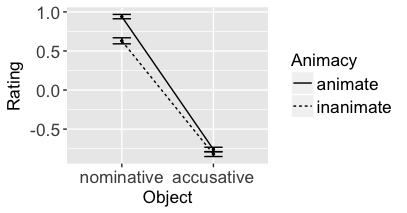
\includegraphics[scale = 0.5]{figures/exp1a_13.png}
\label{fig:exp1a}
\end{figure}

For the statistical analysis, a mixed-effects linear model was constructed using the \texttt{lmer} function from the R statistical language package \texttt{lmerTest}. The model included the factors \textsc{construction type} and \textsc{animacy} as well as their interaction as fixed effects and had a maximal random effects structure (including random intercepts for subject and item as well as by-item and by-subject random slopes, and correlations for all fixed effects and their interaction), as recommended by \citet{Barr.Levy2013}. $p$-values were obtained using the Satterthwaite approximation, available from the same package.\footnote{The statistical procedures followed \citet{Keshev.meltzerAsscher2019}.}

As expected, there was a highly significant main effect of \textsc{construction type}, showing that sentences with \textsc{acc} themes are rated lower than sentences with \textsc{nom} themes ($\text{Estimate} = -1.70$, $\text{SE} = 0.04$, $t = -29.1$, $p < 0.001$). There was~also a main effect of \textsc{animacy}, showing that sentences with inanimate subjects are rated lower than sentences with animate subjects ($\text{Estimate} = -0.31$, $\text{SE} = 0.12$,  $t = -2.59$, $p = 0.03$), although this effect was less significant. However, the interaction was not significant ($\text{Estimate} = 0.24$, $\text{SE} = 0.12$, $t = 2.02$, $p = 0.08$). Interestingly, the (trend towards an) interaction was not in the predicted direction as inanimacy turned out to decrease rather than increase the lowering effect of the construction with \textsc{acc}. This pattern has been noted before in the experimental syntax literature and has come to be identified as a \textsc{subadditive} effect (see, e.g., \citealt{Stepanov.Music.Stateva2018}).

\subsubsection{Discussion}

As it stands, the results of the experiment do not support the hypothesized animacy restriction in the `need'\,+\,\textsc{acc} construction, calling for an explanation. Note first that a floor effect is unlikely, as the ungrammatical fillers received a ($z$-score) rating of $-0.98$, which is $0.23$ points lower than the \textsc{acc} | \textsc{inanimate} condition ($-0.75$). However, there might be an alternative source of the negative results.

Given a very large effect of the \textsc{construction type} (the lowering effect of $-1.7$ points in the animate condition), it is likely that the participants judged the `need'\,+\,\textsc{acc} construction as simply ungrammatical; see the raw rating of $1.8$--$1.98$ for the two \textsc{acc} conditions. It has been suggested in the processing literature \citep[see][]{Hofmeister.Casasanto.Staum.Sag2014} that when one grammatical violation combines with another grammatical violation or a processing effect, the result may be subadditive (underadditive) rather than additive or superadditive, whereby the second grammatical violation or a processing difficulty does not lead to a further decrease in unacceptability in the ungrammatical condition. I tentatively suggest that this is what might have happened in this experiment.

Specifically, given the perceived strong ungrammaticality of the `need'\,+\,\textsc{acc} construction, I suggest that an additional violation of the animacy restriction caused no further decrease in acceptability and thus failed to be detected. Similarly, the processing effect of animacy, which we observe in the `grammatical' \textsc{nom} condition, did not show up in the ``ungrammatical'' \textsc{acc} condition, presumably leading to a trend towards a sub-additive interaction.

\subsection{Experiment 1b}

\subsubsection{Design and materials}

Experiment 1b had the same purpose as Experiment 1a but a slightly different design with materials constructed in such a way as to increase the overall ratings of the `need'\,+\,\textsc{acc} construction (and potentially reduce its perceived ungrammaticality). A prior corpus study established that the `need'\,+\,\textsc{acc} construction has a higher absolute frequency with \textit{nado} than with \textit{nužno}.\footnote{We cannot compare relative frequencies as \textit{nado} is disallowed in the `need'\,+\,\textsc{nom} construction.} Accordingly, it was decided to use \textit{nado} in the \textsc{acc} condition. Furthermore, it was observed that dative subjects realized as full NPs are very rare in the construction, compared to pronominal NPs. Accordingly, 3rd person pronouns (both singular and plural) were used as dative subjects. Although they are not as frequent as the 1st person singular pronoun (which is the most frequent one), this allowed to have more variety in the materials. In order to fix the reference of the pronominal subject, the experimental sentences were preceded by a supporting context consisting of a short sentence with one prominent referent, either animate or inanimate. The materials for the experiment are illustrated in \REF{materials-exp1b-anim} and \REF{materials-exp1b-inan}.

\ea \label{materials-exp1b-anim} \gll \textit{Context}: U Kati slomalsja noutbuk.
\\
{} at Katja broke laptop\\
\glt \hspace{1.3cm} `Katja's laptop broke down.'\\
\ea \gll Ej nužen adapter.\\
her.\textsc{dat} necessary.\textsc{m.sg} adapter.\textsc{nom.sg}\\ \hfill \textsc{nom} | \textsc{animate}
\glt `She needs an adapter.'
\ex \gll Ej nado adapter.\\
her.\textsc{dat} necessary.\textsc{adv} adapter.\textsc{acc.sg}\\ \hfill \textsc{acc} | \textsc{animate}
\glt `She needs an adapter.'
\z \ex \label{materials-exp1b-inan} \gll \textit{Context}: Ėtot noutbuk slomalsja.\\
{} this laptop broke\\
\glt \hspace{1.3cm} `This laptop broke down.' \\
\ea[]{\gll Emu nužen adapter.\\
him.\textsc{dat} necessary.\textsc{m.sg} adapter.\textsc{nom.sg}\\ \hfill \textsc{nom} | \textsc{inanimate}
\glt `It (the laptop) needs an adapter.'}
\ex[*]{\gll Emu nado adapter.\\
him.\textsc{dat} need.\textsc{adv} adapter.\textsc{acc.sg}\\ \hfill \textsc{acc} | \textsc{inanimate}
\glt Intended: `It (the laptop) needs an adapter.'}
\z\z

\noindent Eight sentence sets of four sentences as in \REF{materials-exp1b-anim} and \REF{materials-exp1b-inan} were constructed. The experimental sentences were distributed over four protocols using a Latin square design and interspersed with 12 filler sentences, which were similar to those used in Experiment 1a except that half of the sentences were with \textit{nado} and there were four sentences of intermediate acceptability that contained inanimate dative subjects with \textit{nado/nužno} followed by infinitival/subjunctive clauses (to contrast the hypothesized animacy restriction with different types of sentences with `need'). The experiment was printed and distributed to philology students at a local university. The task and instructions were as in Experiment 1a. Seventy-one students participated in the experiment.

\subsubsection{Results}

The data from two students were discarded due to missing values. The analysis of the data used $z$-score transformed ratings, as in Experiment 1a. The mean rating for the ungrammatical fillers was $-0.96$ ($\text{SD} =0.56$); the mean rating for the grammatical fillers was $0.97$ ($\text{SD} =0.46$); the mean rating for the intermediate fillers was $0.08$ ($\text{SD} =0.79$). The raw ratings were $1.66$ ($1.48$),  $6.40$ ($1.17$) and $3.85$ ($2.07$), respectively. The condition means are given in \tabref{tab:1:means-exp1b} and in \figref{fig:exp1b}.\largerpage

%\begin{table}
%\caption{Z-score means (SD) in Experiment 1b}
%\label{tab:1:means-exp1b}
% \begin{tabular}{lllll}
 % \lsptoprule
  %          & \textsc{need\,+\,nom} & \textsc{need\,+\,acc}\\
 % \midrule
 % animate  &   1.01 (0.50) &   --0.46 (0.64)\\
 % inanimate  &   0.38 (0.77) &   --0.80 (0.46)\\
% animate (raw)  &   6.46 (1.23) &   2.86 (1.83)\\
%  inanimate (raw)  &   5.01 (1.98) &   2.09 (1.28)\\
%  \lspbottomrule
 %\end{tabular}
%\end{table}

\begin{table}
\centering
\begin{tabular}{lrr}
\lsptoprule
   & `need'\,+\,\textsc{nom} & `need'\,+\,\textsc{acc}\\
\midrule
animate  &  $1.01$ ($0.50$) &   $-0.46$ ($0.64$)\\
inanimate  & $0.38$ ($0.77$) &   $-0.80$ ($0.46$)\\
animate (raw)  &   $6.46$ ($1.23$) &  $2.86$ ($1.83$)\\
inanimate (raw)  &   $5.01$ ($1.98$) & $2.09$ ($1.28$)\\
\lspbottomrule
\end{tabular}
\caption{$z$-score means (SD) in Experiment 1b}
\label{tab:1:means-exp1b}
\end{table}

\begin{figure}
\caption{Interaction plot for Experiment 1b}
\centering
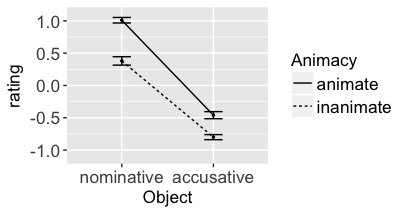
\includegraphics[scale = 0.5]{figures/exp1b_13.png}
\label{fig:exp1b}
\end{figure}

There was a main effect of construction type ($\text{Estimate} = -1.46$, $\text{SE} = 0.15$, $t = -9.23$, $p < 0.001$), showing that sentences with \textsc{acc} themes are rated lower than sentences with \textsc{nom} themes and a main effect of \textsc{animacy}, showing that sentences with inanimate subjects are rated lower than sentences with animate subjects ($\text{Estimate} = -0.62$, $\text{SE} = 0.15$, $t = -4.09$, $p = 0.003$). The effect of animacy was more significant and more reliable than in Experiment 1a. The interaction, however, was not statistically significant and numerically in the opposite direction, as in Experiment 1a ($\text{Estimate} = 0.29$, $\text{SE} = 0.17$, $t = 1.74$, $p = 0.12$).

\subsubsection{Discussion}

The results of Experiment 1b were similar to those of Experiment 1a. Modifications in the design, however, did bring some change in the pattern of the results. The mean rating for the \textsc{acc} | \textsc{animate} condition, which can be used to assess whether speakers perceived the `need'\,+\,\textsc{acc} construction as grammatical (in the absence of hypothesized selectional violations), was higher ($-0.46$) than in Experiment 1a ($-0.69$); compare $2.86$ with $1.8$ in raw ratings, and somewhat closer to intermediate acceptability. This suggests that in absolute terms participants did not perceive the `need'\,+\,\textsc{acc} construction as totally ungrammatical; compare $-0.96$ for the ungrammatical fillers with $1.66$ in raw ratings.

In relative terms, however, the decrease associated with the \textsc{acc} (in the \textsc{animate} condition) was still very strong ($-1.46$, as compared to $-1.62$ in Experiment 1a). Therefore, it is likely that participants still perceived the `need'\,+\,\textsc{acc} construction as ungrammatical, which, again, may have led to a failure to detect the animacy restriction, as in Experiment 1a. Thus, the negative results of Experiment 1b are also consistent with the assumption that combined violations involving grammatical violations do not necessarily add up to decrease the overall acceptability of the sentence. Overall, the main difference between Experiments 1a and 1b was that the participants in the second experiment were more sensitive to the animacy manipulation in the \textsc{nom} condition, which gave rise to a more pronounced animacy effect.

\subsection{Experiment 2}

\subsubsection{Design and hypotheses}

The purpose of Experiment 2 was to test the concreteness restriction on the \textsc{acc} argument in the `need'\,+\,\textsc{acc} construction with \textit{nužen}/\textit{nužno}. The experiment had a 2\times 2 factorial design, crossing the \textsc{construction type} and \textsc{concreteness} (\textsc{concrete} | \textsc{abstract}), as illustrated in \REF{materials-exp2-anim} and \REF{materials-exp2-inan}. The hypothesis was that both \textsc{acc} marking and abstractness will lower acceptability. As in Experiments 1a and 1b, it was also expected that the lowering effect of \textsc{acc} will be stronger in the abstract condition, leading to a superadditive interaction.

\ea \gll \textit{Context}: U Kati peregorel svet. \label{materials-exp2-anim}\\
{} at Katja burn.out light\\
\glt \hspace{1.3cm} `The lights burned out at Katja's place.'
\ea[]{ \gll Ej nužn-a lampočk-a.\\
her.\textsc{dat} necessary-\textsc{f.sg} lightbulb-\textsc{nom.sg}\\ \hfill \textsc{nom} | \textsc{concrete}
\glt `She needs a lightbulb.'}
\ex[]{ \gll Ej nužno lampočk-u.\\
her.\textsc{dat} necessary.\textsc{adv} lightbulb-\textsc{acc.sg}\\ \hfill \textsc{acc} | \textsc{concrete}
\glt `She needs a lightbulb.'}
\z \ex \gll \textit{Context}: Katja ne možet sama rešit' ėtu problemu. \label{materials-exp2-inan}\\
{} Katja not can self solve this problem\\
\glt \hspace{1.3cm} `Katja can't solve this problem alone.'
\ea[]{\gll Ej nužn-a konsul'taci-ja.\\
her.\textsc{dat} necessary-\textsc{f.sg} advice-\textsc{nom.sg}\\ \hfill \textsc{nom |  \textsc{abstract}}
\glt `She needs advice.'}
\ex[*]{\gll Ej nužno konsul'taci-ju.\\
her.\textsc{dat} necessary.\textsc{adv} advice-\textsc{acc.sg}\\ \hfill \textsc{acc} | \textsc{abstract}
\glt Intended: `She needs advice.'}
\z\z

\subsubsection{Materials and procedure}

 The construction of materials was as in Experiment 1b except that the modal predicate did not vary within the sentence sets. As before, there were eight sentence sets of four conditions as in \REF{materials-exp2-anim} and \REF{materials-exp2-inan}. The abstract/concrete nouns within a sentence set were matched in gender, length, and frequency (according to \citealt{Ljasevskaja.Sarov2009}). The experimental sentences were interspersed with eight fillers similar to those in Experiment 1a. The task was as in the two previous experiments except that a 5-point rating scale was used. The experiment was conducted in Google Forms and was completed by 54 participants.

\subsubsection{Results}

The analysis followed the same procedure as in the previous experiments. The mean rating for the ungrammatical fillers was $-1.07$ ($\text{SD} =0.42$); the mean rating for the grammatical fillers was $0.81$ ($\text{SD} =0.43$). The raw ratings were $1.19$ ($0.68$) and $4.57$ ($0.84$), respectively. The condition means are given in \tabref{tab:1:means-exp2} and in \figref{fig:exp2}. %change to SD everywhere

%\begin{table}
%\caption{Z-score means (SD) in Experiment 2}
%\label{tab:1:means-exp2}
% \begin{tabular}{lllll}
 % \lsptoprule
  %          & \textsc{need\,+\,nom} & \textsc{need\,+\,acc}\\
 % \midrule
 % concrete  &   0.89 (0.45) &   --0.43 (0.55)\\
 % abstract  &   0.79 (0.54) &   --0.71 (0.51)\\
 % concrete (raw)  &   4.72 (0.84) &   2.31 (1.23)\\
 % abstract (raw) &   4.53 (1.04) &   1.81 (1.09)\\
 % \lspbottomrule
 %\end{tabular}
%\end{table}

\begin{table}
\centering
\begin{tabular}{lrr}
\lsptoprule
   & `need'\,+\,\textsc{nom} & `need'\,+\,\textsc{acc}\\
\midrule
concrete  &   $0.89$ ($0.45$) &   $-0.43$ ($0.55$)\\
abstract  &   $0.79$ ($0.54$) &   $-0.71$ ($0.51$)\\
concrete (raw)  &   $4.72$ ($0.84$) &   $2.31$ ($1.23$)\\
abstract (raw) &   $4.53$ ($1.04$) &   $1.81$ ($1.09$)\\
\lspbottomrule
\end{tabular}
\caption{$z$-score means (SD) in Experiment 2}
\label{tab:1:means-exp2}
\end{table}

\begin{figure}
\caption{Interaction plot of $z$-score ratings (SE) for Experiment 2}
\centering
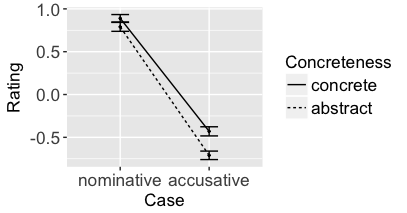
\includegraphics[scale = 0.5]{figures/exp2_13.png}
\label{fig:exp2}
\end{figure}

There was a main effect of construction type ($\text{Estimate} =-1.32$, $\text{SE} =0.11$, $t = -12.5$, $p < 0.001$), showing that sentences with \textsc{acc} themes were rated lower than sentences with \textsc{nom} themes, as in the previous experiments. Neither the main effect of concreteness ($\text{Estimate} =-0.07$, $\text{SE} =0.13$, $t$ = $0.59$, $p$ = $0.58$) nor the interaction between concreteness and construction type ($\text{Estimate} =-0.23$, $\text{SE} =0.16$, $t$ = $-1.44$, $p$ = $0.19$) were statistically significant. Although the interaction was not significant, we see a trend in the predicted direction, in contrast to Experiments 1a and 1b. Moreover, the size of the interaction ($-0.23$) is close in magnitude to the lower boundary for weak islands effects as reported by \citet{Kush.Lohndal.Sprouse2018}.

\subsubsection{Discussion}

As in the case with the animacy restriction in Experiments 1a and 1b, the results of Experiment 2 failed to provide support for the hypothesized concreteness restriction. However, given a very strong lowering effect of \textsc{acc} ($-1.32$; compare $-1.62$ with $-1.46$ in the previous experiments), it may again be hypothesized that the participants perceived the `need'\,+\,\textsc{acc} construction as ungrammatical. Given the explanation suggested for Experiments 1a and 1b above, according to which grammatical violations need not combine additively, this may have led to the lack of a statistically significant interaction in the results and thus a failure to detect the concreteness restriction. Interestingly, in contrast to Experiments 1a and 1b, there was no independent effect of concreteness, suggesting that abstractness of the \textsc{acc} theme did not incur any extra processing costs (in the \textsc{nom} condition). This might have led to the absence of a subadditive pattern which was observed in Experiments 1a and 1b.

\subsection{General discussion}

Unfortunately, the three experimental studies reported above failed to confirm the animacy and concreteness restrictions in the `need'\,+\,\textsc{acc} construction (as operationalized by the presence of superadditive interactions) and thus do not provide (indirect) evidence for the analysis of this construction as involving the control relation (syntactically represented as the Ctr head), which was proposed in \sectref{section-acc-analysis}.

However, this does not necessarily imply that the proposed account of the `need'\,+\,\textsc{acc} construction is wrong. As I suggested above, the failure to obtain superadditive interactions in the experiments could be due to the perceived ungrammaticality of the `need'\,+\,\textsc{acc} construction. This may have nullified the lowering effect of the selectional violations associated with the control relation (i.e., the animacy and concreteness restrictions), in accordance with the hypothesis that grammatical violations may not combine additively, as argued in \citet{Hofmeister.Casasanto.Staum.Sag2014}.

This interpretation, of course, requires investigation. Further studies will have to find ways to eliminate the supposed ungrammaticality effect. One obvious possibility is to try to use oral materials to bias participants away from the written/standard variant.\footnote{This was suggested to me by Diogo Almeida (p.c.).} Another option is to alter the judgment task, in view of the possibility that subjects might find it difficult to discriminate between different types of ungrammatical sentences on a scale. For example, one might try using relative judgments with the Thurstone model \citep[see][]{Langsford.etal2018} or a joint presentation of conditions, as suggested by \citet{Marty.Chemla.Sprouse2020}.

All in all, the basic prediction of the proposed account is that a superadditive interaction will become visible once the participants are able to judge the `need'\,+\,\textsc{acc} construction as acceptable.

\section{Conclusion\label{section-conclusion}}

In this paper, I have discussed two `need'\,+\,NP constructions in \ili{Russian}, namely, the more basic `need'\,+\,\textsc{nom} construction and the more marginal, highly colloquial `need'\,+\,\textsc{acc} construction. The main focus was on the contrast in the semantic variability between these two constructions (i.e., the range of relations that they can express), as discussed by \citet{Zaroukian.Beller2013} with reference to English transitive `need' and related constructions.

Specifically, I showed that the `need'\,+\,\textsc{nom} construction in \ili{Russian}
can express a variety of relations, including the (arguably most prototypical) control relation, but also the inherent, part-whole, and typical-use relations, on a par with English transitive `need'. I also identified two new relations which have not been discussed before in this connection, namely the thematic relation (expressed in constructions with deverbal nominals) and the requirement relation, which are compatible with both `need'\,+\,\textsc{nom} and English transitive `need'. I also showed that, crucially, in contrast to the `need'\,+\,\textsc{nom} construction (and transitive `need'), the `need'\,+\,\textsc{acc} construction is restricted to the expression of the control relation. This is suggested by the presence of the concreteness and animacy restrictions (which are lexically associated with the control relation) in this construction.

\begin{sloppypar}
I proposed an analysis of the two `need'\,+\,NP constructions in \ili{Russian} whereby they both take a concealed clausal complement involving silent \textsc{have}, as was proposed in the previous literature on intensional transitive verbs \citep[e.g.,][]{Harves2008}. However, in contrast to the previous literature, I used a more elaborate analysis of the semantic variability associated with \textsc{have}. Specifically, I followed \citet{Zaroukian.Beller2013}, where diverse \textsc{have}-relations are modeled as various (syntactically represented) type-shifters, which provide relational denotations for the object NP, whereas \textsc{have} is treated as an abstract linker between the subject NP and the NP-relation.
\end{sloppypar}

In order to capture the contrast in the semantic variability between the `need'\,+ \textsc{nom} construction and the `need'\,+\,\textsc{acc} construction, I argued that the latter but not the former incorporates (via head movement) the type-shifter associated with the control relation (i.e., Ctr). I also tentatively suggested that this might explain the \textsc{acc} marking in the `need'\,+\,\textsc{acc} construction along the lines of the P-incorporation account of `have' in \citet{Freeze1992} \citep[see also][]{Kayne1993}.


Finally, I discussed three acceptability judgment studies, which used a factorial design to test the animacy and the concreteness restriction in the `need'\,+\,\textsc{acc} construction, which are associated with the control relation. Intriguingly, these studies failed to provide support for these restrictions (experimentally operationalized as a superadditive interaction). I speculated that the negative results might be due to the perceived ungrammaticality of the `need'\,+\,\textsc{acc} construction and the hypothesis that combined grammaticality violations may not add up to decrease the overall acceptability (see \citealt{Hofmeister.Casasanto.Staum.Sag2014} for further discussion). This suggestion must, of course, be tested in future work.

\section*{Appendix: Experimental materials}

\ea Items for Experiment 1a
\ea Voditeljam (avtomobiljam) nužen (nužno) benzin.
\ex  Voennym (samoletam) nužen (nužno) aėrodrom.
\ex  Stroiteljam (betonu) nužna voda (nužno vodu).
\ex  Juveliru (kamnju) nužna oprava (nužno opravu).
\ex  Škol'niku (smartfonu) nužen (nužno) modnyj čexol.
\ex  Žil'cam (komnate) nužny (nužno) svetlye oboi.
\ex  Klientu (noutbuku) nužen (nužno) akkumuljator.
\ex  Znakomym (knigam) nužen (nužno) stellaž.
\z \ex Items for Experiment 1b
\ea Ej (=\,Maše)\slash emu (=\,telefonu) nužen (nado) čexol.
\ex Ej (=\,Kate)\slash emu (=\,noutbuku) nužen (nado) adapter.
\ex  Im (=\,sosedjam)\slash ej (=\,komnate) nužna ljustra (nado ljustru).
\ex  Im (=\,sotrudnikam)\slash im (=\,oknam) nužny\slash nado žaljuzi.
\ex  Nam\slash emu (=\,avtomobilju) nužen (nado) voditelja.
\ex  Im (=\,organizatoram)\slash ej (=\,olimpiade) nužny volontery\slash nado volonterov.
\ex  Ej (=\,Svete)\slash im (=\,glazam) nužen (nado) otdyx.
\ex  Nam\slash emu (=\,kišečniku) nužna podderžka (nado podderžki).
\z \ex Items for Experiment 2
\ea Ej nužna kletka (podderžka)\slash nužno  kletku (podderžku).
\ex Emu nužen\slash nužno  orden (otpusk).
\ex Ej nužna figurka (uborka)\slash nužno  figurku (uborku).
\ex Emu nužen\slash nužno  kostjum (povod).
\ex Ej nužna lampočka (konsul'tacija)\slash nužno  lampočku (konsul'taciju).
\ex Ej nužna svekla (otsročka)\slash nužno  sveklu (otsročku).
\ex Ej nužna pižama (razrjadka)\slash nužno  pižamu (razrjadku).
\ex Ej nužna ručka (družba)\slash nužno  ručku (družbu).
\z \z

\section*{Abbreviations}

\begin{tabularx}{.5\textwidth}{@{}lX}
RNC & Russian National Corpus\\
\textsc{1} & first person\\
\textsc{3} & third person\\
\textsc{adv} & adverbial\\
\textsc{acc} & accusative\\
\textsc{dat} & dative\\
\textsc{f} & feminine\\
\end{tabularx}%
\begin{tabularx}{.5\textwidth}{lX@{}}
\textsc{gen} & genitive\\
\textsc{m} & masculine\\
\textsc{n} & neuter\\
\textsc{nom} & nominative\\
\textsc{pl} & plural\\
\textsc{sg} & singular\\
\textsc{sbjv} & subjunctive\\ % here and in glosses > sbjv (according to LGR)
\end{tabularx}


\section*{Acknowledgements}

I wish to thank the audiences of FDSL\,13 at the University of Göttingen (December 5--7, 2018) and the 15th Conference on typology and grammar for young researchers at the Institute for Linguistic Studies, RAS (November 22--24, 2018) for their valuable comments and suggestions. I also thank two anonymous reviewers for their helpful feedback on the manuscript.

{\sloppy\printbibliography[heading=subbibliography,notkeyword=this]}
\end{document}
